\chapter{Literature Review}\label{chapter:literature_review}

\section{Message Passing Paradigm}
\label{sec:messagePassing}
  Message passing is simply sending a message from one process, component or actor to another. The recipient of the message chooses further processing based on the pattern or content of the message.
  Message passing is the loosest type of coupling. The components of a system are not dependent on each other; instead they use a public interface to exchange parameterless messages\cite{joecelko}. Hence, systems that implement message passing paradigm are easily scalable and efficient. Such systems are easy to replicate and thus fault tolerance can be improved~\cite{Armstrong:2010:ERL:1810891.1810910}.

  The systems which communicate solely by message passing do not have a shared state. Such systems can be easily divided into isolated components. This makes the overall architecture of a system easy to understand and simplifies the separation of problems within the system~\cite{Armstrong:2010:ERL:1810891.1810910}.

  Message passing can either be synchronous or asynchronous. Synchronous message passing is the communication between two components where both the sender and the receiver of a message are ready to communicate. As the sender of a message has to wait for a response from the receiver, the sender is usually blocked until it gets a reply. Whereas, in asynchronous message passing, the sender simply sends a message and carries on with further processes. The receiver does not have to be ready to accept the message when the sender sends it.~\cite{agha} Thus, an asynchronous message passing is non-blocking in nature.

\section{Actor Programming Model}
\label{sec:actorProgramming}
  Actor programming model is a programming paradigm designed for concurrent computation. The concept of an actor was originally introduced by Carl Hewitt\cite{hewitt} and he along with Agha\cite{agha} have been involved in development of both the actor theory as well as its implementation.

  An actor is a fundamental unit of computation. It is neither an operating system process nor a thread, but a lightweight process. It embodies three essential things:
\begin{itemize}
  \item Processing
  \item Storage
  \item Communication
\end{itemize}
  Actors have addresses and there is a many-to-many relationship between actors and addresses. i.e Each actor can have multiple addresses and multiple addresses can belong to one actor.

  Actors communicate with each other in a non-blocking way by asynchronous message passing, which removes the need of explicit locks. An actor can send message to actors in same system or another system. An actor can also send message to itself, which is how a recursion is achieved. An actor can send a message to target actor only if it has the address of target actor. Agha~(\cite{agha}, p35) lists three ways in which an actor, upon accepting a message, can know the address of the target actor:
  \begin{itemize}
    \item the target was known to the actor a before it accepted the message
    \item the target became known when the message was accepted because it was contained in the message, or,
    \item the target is the new actor created as a result of accepting the message
  \end{itemize}

  To buffer incoming messages, each actor has a mailbox. A mailbox is a queue of messages that have been sent by other actors or processes and not yet consumed, where mailbox is also an actor. The order in which the messages are delivered is non-deterministic~\cite{hewittVideo}.

After receiving a message, an actor may perform following actions.~\parencite{hewitt}
\begin{itemize}
  \item Create other actors
  \item Send messages to itself, other known actors or reply to the actor who sent the message
  \item Designate how it is going to handle next message, i.e. Specify a replacement behavior
\end{itemize}

Actors do not have a shared mutable state. All mutable state is private to the actor and all shared state is immutable. Actors communicate with each other by asynchronous message passing which is also immutable. Each actor processes only one message at a time, and unless it is a broadcast message, a message is not processed multiple times.

  An actor exists in a system. An actor system is a group of actors working together in certain hierarchy.
  In the actor model, concurrency is inherent because of the way it is designed. Also, there is no guarantee that the message sent to an actor will arrive sequentially~\cite{hewittVideo}.

  Several programming languages like Act 1, 2 and 3, Acttalk etc. were created when actor system was newly introduced by Hewitt and Agha~\cite{agha, hewitt}.

\subsection{Error Handling in Actor Model}
Exception handling in actor model is based on idea of embracing the failures. The idea of embracing failures is also known as “let it crash” paradigm~[\autoref{subsec:letItCrash}]. As the actors do not have shared state, this allows individual actor to fail without causing disruptions in the system. Since, an actor in an actor system is typically organized in a hierarchical structure, the actor which created a child actor can be used for supervising it. The idea of supervision in a hierarchical actor system helps to make the actor system fault tolerant~\cite{Erb2012}. When an actor throws an exception the supervisor can respond to the exception in different ways. In Akka~[\autoref{sec:akka}], the supervising actor usually reacts by either simply ignoring the exception and let the actor continue, restarting the actor or by escalating the error to its supervisor.

  The “let it crash” style of programming is a non-defensive programming, which is implemented successfully in Erlang~[\autoref{sec:erlang}].

\subsection{Differences from thread-based programming model}
\subsubsection{Thread-based Concurrency}
  \label{subsec:thread}
  In thread-based programming languages, the control flow of a program is divided into several threads for concurrency. The threads operate simultaneously and the control can switch from one thread to another non-deterministically. When two or more threads have a shared memory, concurrent modifications and accesses of the data might result in undesired behavior of the system, known as ‘race condition’. To prevent this type of situations, such programming languages have locks. The locks let only a single thread at a time to run sequentially for a section of program code~\cite{ambientTalk}.

  Generally, the thread-based programming models are easy to understand and implement. But, the resulting program behavior is difficult to understand because of implicit context switches and release of locks, which may even lead to a deadlock situation~\cite{ambientTalk}.

\subsubsection{Actors based Concurrency}
\label{subsec:actorConcurrency}
  Concurrency in actor based programming languages are inherent because of using asynchronous message-passing, pipelining, and the dynamic creation of actors.
The concurrency in actors through pipelining is only constrained by the logical limits and the available hardware resources~\cite{agha}. The actors may carry out their activities in parallel as each actor resides in a completely separated space from the other actors, they are connected only via messages.

  The actor based programming liberates the programmer from going into coding details about the parallelism and threads~\cite{agha}.

  As actors do not have shared state, thus the ‘race condition’ as discussed in \autoref{subsec:thread}, do not arise in actor based programming.

\subsection{Scaling up actor based systems}
  As actor based systems are highly concurrent~[\autoref{subsec:actorConcurrency}], it is easy to scale actor based systems from a single core system to several of them across multiple data centers around the globe. The ideal case would be to just let a new system join the actor system and let it run some more actors during runtime, without the need of taking down the running system. The actors themselves do not need to know the physical location of other actors as they simply exchange messages based on the logical addresses. This makes them easy to scale up and out.

\section{Erlang}
\label{sec:erlang}
  Erlang is the first popular programming language that was based on the actor model\cite{vinoski}. It was developed by Joe Armstrong in 1986 at the Ericsson Computer Science Laboratory and was made open-source in 1998. It was chiefly used in telephony applications as it was built to solve the problems of availability as well as scalability that existed in such applications.~\parencite{armstrong}

  Erlang ‘processes,’ which are essentially user-space threads rather than Unix processes or kernel threads, communicate only via message passing.

  Erlang was designed for the writing applications that require high availability - as Armstrong mentions it in his \cite{armstrong} the programs that “run forever”. It uses concurrent processes, which have no shared memory and communicate only via asynchronous message passing. This idea is similar to the actors model proposed by Agha and Hewitt~\autoref{sec:actorProgramming}. Thus, programs written in Erlang are concurrent, distributed, fault tolerant and thread safe. The concurrency is built into the language itself, not the the operating system~\cite{Armstrong:2010:ERL:1810891.1810910}.

  When an application developed in Erlang is deployed in a multicore computer, it automatically takes advantage of those multiple cores. The Erlang “processes” spread over the cores and so the programmers do not have to worry about threads~\cite{Armstrong:2010:ERL:1810891.1810910}. Erlang has mechanisms to let the programs update themselves without taking the system offline. The new changes in an application can be added while the system is up, which improves the availability of whole system. Thus, simplifying the construction of software for implementing non-stop systems~\cite{armstrong}.

  Error handling in Erlang is different from most of the other programming languages. The error handling is based on a “let it crash” philosophy~\autoref{subsec:letItCrash} which is a non-defensive style of programming~\cite{armstrong, Armstrong:2010:ERL:1810891.1810910}.

\subsection{“Let it Crash” Philosophy}
\label{subsec:letItCrash}
  The core idea in “Let it Crash” philosophy is to let the failing processes crash and make other processes, which observe this process, detect the crashes and fix them~\cite{Armstrong:2010:ERL:1810891.1810910}. This idea is in sharp contrast to other programming languages, where programmers implement exception handlers and prevent a process from getting terminated.

  The concept of “let it crash” leads to clear and compact coding
~\cite{Armstrong:2010:ERL:1810891.1810910}.

\section{Scala Actors}
Scala is a statically typed programming language which integrates functional as well as object-oriented programming\cite{Odersky}. Scala has its own library for actor programming.

  In Scala, templates for actors with user-defined behavior are normal class definitions which extend the predefined Actor class.

  The scala actors library provide concurrent programming model based on actors~[\autoref{sec:actorProgramming}]. The actors in scala are fully inter-operable with the mainstream virtual machine threads~\cite{Haller}. Scala actors are lightweight and support around 240 times more actors to run simultaneously compared to virtual machine threads~\cite{Haller}.

  Both synchronous and asynchronous message passing can be used to in scala actors. The synchronous message passing is implemented by exchanging several asynchronous messages. The actors in scala can also communicate using ‘futures’. When a future is used the requests are handled asynchronously and the sender immediately gets a representation of the future which allows sender to wait for the reply.~\cite{scalaActors}

  The Scala Actors library is now deprecated and will be removed in future Scala releases\footnote{Scala actors are deprecated in version 2.10, \fullcite{scalaActorsAPI}}. The deprecation is in favor of the use of Akka actors~[\autoref{sec:akka}].

\section{Akka Toolkit}
\label{sec:akka}
Akka is a toolkit and runtime for building highly concurrent, distributed and resilient message-drive applications on the JVM. Akka uses lightweight actors for concurrency. The actors in Akka are based on Hewitt's and Agha's model~\cite{agha, hewitt} of actor programming. Akka provides a well defined API for developers to develop large concurrent systems, which allows for easy scaling out.
  Akka is available for Scala as well as Java.

  \subsection{Actor Model in Akka}
  In Akka, actors are objects which encapsulate state and behavior. Similar to Hewitt's and Agha's actor model~[\autoref{sec:actorProgramming}], the akka actors communicate only by message sending which are placed into the recipient’s mailbox. Akka actors are the stringent form of object-oriented programming~\cite{akkaActorSystem}.

  The ‘ActorRef’ in akka, represents an actor. It holds a reference to an actor. Its purpose is to facilitate the message sending to the actor it refers. An actor can also refer to itself using \emph{self}. ~\cite{akkaJavaDoc}

  The \autoref{lst:akkaHelloWorld}~\footnote{Source: \fullcite{akkaHome}}, is a simple example of how actor programming in Akka is realized. In this example, the ‘GreetingActor’ is an actor which extends ‘UntypedActor’ must implement the \emph{onReceive()} method. The \emph{onReceive()} method is invoked for each message that is received by this actor. After receiving a message, the actor performs pattern matching to decide which code to execute. As in this example, if the message is a type of ‘Greeting’ object, it is concatenated with the string “Hello” otherwise, it is simply ignored.

\begin{lstlisting}[caption=A simple example of actor programming in akka~\cite{akkaHome}, label=lst:akkaHelloWorld]
public class Greeting implements Serializable {
  public final String who;
  public Greeting(String who) { this.who = who; }
}

public class GreetingActor extends UntypedActor {
  LoggingAdapter log = Logging.getLogger(getContext().system(), this);

  public void onReceive(Object message) throws Exception {
    if (message instanceof Greeting)
      log.info("Hello " + ((Greeting) message).who);
    }
}

ActorSystem system = ActorSystem.create("MySystem");
ActorRef greeter = system.actorOf(Props.create(GreetingActor.class), "greeter");
greeter.tell(new Greeting("Charlie Parker"), ActorRef.noSender());
\end{lstlisting}


  \subsection{Actor System}
      An actor system in Akka is like an organization of actors where actors are arranged in a hierarchical structure. An actor, which performs certain task usually split up the task into smaller pieces. For this, it starts up other actors as its child actors, which it supervises~\autoref{subsec:supervisionMonitoring}. As the actor which creates a new actor is the supervisor of the new actor, it is implicit that there can be only one supervisor of an actor.

  By splitting up the tasks, the tasks become clear and structured. Furthermore, the resulting actors also becomes simplified and specialized in terms of which messages it should process and how it should react normally. It also becomes easy to handle the failures. If an actor cannot cope with a failure, it is escalated up in the hierarchy to its supervisor which is recursive unless it reaches up to the actor which can handle the failure.~\cite{akkaJavaDoc}

  An actor instance in akka takes up roughly 300 bytes of memory, because of which it is possible to spawn millions of them in one actor system. As an actor system can grow very large and distributed, the order of message processing is not guaranteed.~\cite{akkaJavaDoc}

  An example of the arrangement of actors in hierarchical structure is shown in~\autoref{fig:actorSystem}. The ‘{$\backslash$}’ is known as the “root guardian” and \emph{$\backslash$user} is known as the “user guradian”. Any actor created by a user falls under the user guradian. For instance, in the~\autoref{fig:actorSystem}, \emph{actorA} and \emph{actorB} are actors created by user, hence their supervisor is \emph{$\backslash$user}. Again, the actors \emph{actor1} and \emph{actor2} are the child actors of \emph{actorB}. The address of an actor in akka is arranged like the filesystem hierarchy. Hence, the supervision hierarchy as well as the path leading to the actor is comprehensible from its address.

\begin{figure}[H]
  \centering
  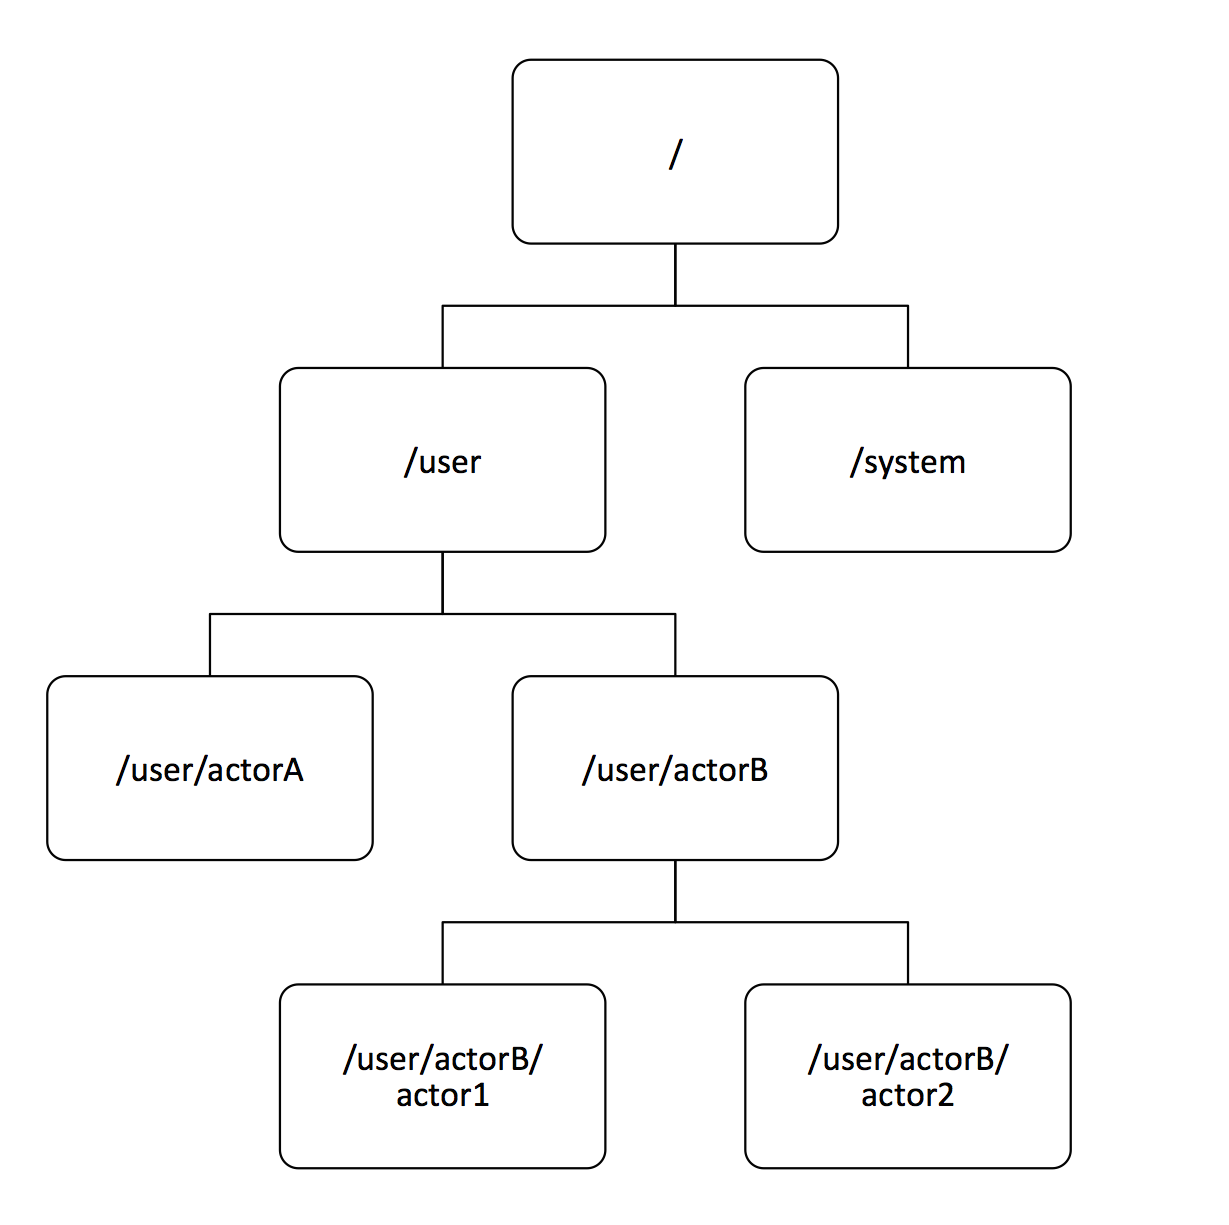
\includegraphics[scale=0.5]{figures/actorSystem}
  \caption[Hierarchy in actor system]{Hierarchy in actor system~\cite{akkaJavaDoc}}
  \label{fig:actorSystem}
\end{figure}

  \subsection{Message Passing in Akka}
  In Akka, every actor has an event driven message inbox known as the ‘mailbox’. The mailbox buffers all the incoming messages until they are processed. When a message is sent from one actor to the other, the reference to the sender (an ActorRef), is automatically added to the message by default. Thus, during the message processing the recipient actor has a reference to the sender actor through the \emph{sender} method.~\cite{akkaJavaDoc}

  Akka guarantees the order of direct message delivery between two actors. It is only applicable when the mailbox implementation in receiver is FIFO mailbox and the communication takes place only between the two actors without the involvement of intermediatory actors. For instance, if an actor A1 sends messages M1, M2 and M3 to actor A2. The message M1 will be delivered before M2 and the message M2 before M3. Meanwhile, if another actor A3 sends messages M4, M5 and M6 to A2 at the same time, the order of message delivery of M4, M5 and M6 will also be sequential. Nevertheless, there is no guarantee that the messages sent by A1 is delivered before the messages from A3; even if all of the messages from A1 were sent before A3 started sending messages to A2. Provided that the message sending from A1 and A3 are independent of each other. ~\cite{akkaJavaDoc}

  The Akka's documentation for Java, the rules mentioned for message sending are: \cite{akkaJavaDoc}
  \begin{itemize}
    \item at-most-once delivery, i.e. no guaranteed delivery
    \item message ordering per sender–receiver pair
  \end{itemize}

Here, ‘at-most-once delivery’ means that a message is either not delivered at all (i.e. lost) or delivered only once. Thus, there is no duplicate delivery of a message.

  \subsection{Shared mutable state}
  Since Akka runs on top of the Java Virtual Machine(JVM), there are some pitfalls that the programmer should be aware enough to avoid, which akka cannot enforce. The messages used to communicate between the actors should be immutable. If it is made mutable and the reference of it is sent by the sender to an actor which resides on same JVM, bugs such as race conditions and even some incomprehensible bugs might appear. Also, the sender method must not be closed over, if the block of code could be run in another thread, for instance sending message to sender actor inside a ‘Future’ block. In such cases, the sender reference must be captured into a local variable first. As the reference and behavior of sender can change over time.~\cite{akkaJavaDoc}

  \subsection{Actor Supervision and Monitoring}
  \label{subsec:supervisionMonitoring}
  The supervising actor in akka delegates tasks to its subordinates. It is also responsible for monitoring them for failures. When a child actor detects a failure, it suspends itself as well as its child actors and sends a message to its supervisor about the failure. According to Akka Java documentation\footnote{\fullcite{akkaJavaDoc}}, upon receiving the failure, the supervisor may opt to perform one of the four choices:~\cite{akkaJavaDoc}
  \begin{enumerate}
    \item Resume the subordinate, keeping its accumulated internal state
    \item Restart the subordinate, clearing out its accumulated internal state
    \item Stop the subordinate permanently
    \item Escalate the failure, thereby failing itself
  \end{enumerate}

  When an actor is restarted by the supervising actor, the message that the actor was processing during the time of failure is lost and is not processed again. However, the messages that were in the mailbox of the actor remains safe and new actor resumes processing the other messages in the mailbox~\cite{akkaJavaDoc}.

  \subsection{Routers}
  Routers are specialized actors that act as a load balancer for the actors that it supervises. Akka provides several built-in routing techniques:~\cite{akkaJavaDoc}
  \begin{itemize}
    \item Round Robin Router
    \item Random Router
    \item Smallest Mailbox Router
    \item Broadcast Router
    \item Scatter Gather First Completed Router
    \item Tail Chopping Router
    \item Consistent Hashing Router
  \end{itemize}

It is also possible to use custom implementation of a router by extending \emph{RoutingLogic} class from Akka's routing library.

  \subsection{Remote Actors in Akka}
  Actors in akka are location transparent; they reside in a logical hierarchy of an actor system through which the physical location of an actor in the network can be determined. The location transparency allows the akka applications to be developed locally but deployed into distributed systems simply by changing configurations.~\cite{akkaJavaDoc}

  Actor systems in akka communicate in a peer-to-peer fashion and it is the foundation for Akka Clustering. Akka's Java Documentation\footnote{~\fullcite{akkaJavaDoc}} lists the two design decisions for remoting:
\begin{enumerate}

  \item Communication between involved systems is symmetric: if system A can connect to system B then system B must also be able to connect to system A independently.

  \item The role of the communicating systems are symmetric in regards to connection patterns: there is no system that only accepts connections, and there is no system that only initiates connections.

\end{enumerate}

A sample Akka Configuration and Code for Remote Actors: \footnote{Source: \fullcite{akkaHome}}

\begin{lstlisting}
  // ------------------------------
  // config on all machines
  akka {
    actor {
      provider = akka.remote.RemoteActorRefProvider
      deployment {
        /greeter {
          remote = akka.tcp://MySystem@machine1:2552
        }
      }
    }
  }

  // ------------------------------
  // define the greeting actor and the greeting message
  public class Greeting implements Serializable {
    public final String who;
    public Greeting(String who) { this.who = who; }
  }

  public class GreetingActor extends UntypedActor {
    LoggingAdapter log = Logging.getLogger(getContext().system(), this);

    public void onReceive(Object message) throws Exception {
      if (message instanceof Greeting)
        log.info("Hello " + ((Greeting) message).who);
    }
  }

  // ------------------------------
  // on machine 1: empty system, target for deployment from machine 2
  ActorSystem system = ActorSystem.create("MySystem");

  // ------------------------------
  // on machine 2: Remote Deployment - deploying on machine1
  ActorSystem system = ActorSystem.create("MySystem");
  ActorRef greeter = system.actorOf(Props.create(GreetingActor.class), "greeter");

  // ------------------------------
  // on machine 3: Remote Lookup (logical home of "greeter" is machine2, remote deployment is transparent)
  ActorSystem system = ActorSystem.create("MySystem");
  ActorSelection greeter = system.actorSelection("akka.tcp://MySystem@machine2:2552/user/greeter");
  greeter.tell(new Greeting("Sonny Rollins"), ActorRef.noSender());
\end{lstlisting}

  \subsection{Clustering in Akka}
  Akka does not have any central point of reference. It uses peer-to-peer based gossip protocol to form a cluster. Thus, there is no single point of failure or single point of bottleneck in the system. But, adding a new member in a distributed system requires significant amount of time because of the nature of the gossip protocol. In a benchmark\footnote{\fullcite{akkaBenchmark}} performed by Patrik Nordwall\footnote{Patrick Nordwall is a developer of Akka at Typesafe}, adding nodes to a cluster of at least 1500 nodes took around 15 to 20 seconds in average.


\section{The Dart Language}
  \subsection{Overview}
  Dart is an open-source, class-based, single-inheritance, pure object-oriented programming language developed by Google~\cite{dartEcma}. Dart language is inspired by Smalltalk, Strongtalk, Erlang, C\# and JavaScript~\cite{sethladd}.

  Dart codes are not compiled before running; the Dart Virtual Machine(VM) reads and executes the source code. Dart provides a homogeneous system that encompass both client as well as server as the Dart VM (Virtual Machine) can be embedded in browsers. A version of Chromium – ‘Dartium’ already has Dart VM built into it~\cite{sethladd}.

  Programs in Dart are optionally typed. They can be executed in two modes checked mode and production mode. In checked mode incorrect static type annotations produce compile time errors. Whereas, in production mode, type annotations are completely ignored~\cite{dartEcma}.

  Furthermore, Dart allows developers to code in a uniform way for both server as well as client since Dart Virtual Machine (VM) can be embedded in browsers. A variant of Chromium browser — Dartium browser has an embedded Dart VM.

  Dart has automatic garbage collecting system, which means the memory occupied by objects which are not in use and which do not have any reference are reclaimed periodically.

  Developers of dart believe that JavaScript has been pushed to its limit and the web apps developed in JavaScript are far too slow even though JavaScript engines are fast. They claim Dart offers a better solution to build larger and more complex web apps\cite{laddWalrath}.

Some of its important features are:
  \begin{itemize}
    \item Easy to learn syntax
    \item Compiles (Translates) to JavaScript
    \item Runs in client as well as on server
    \item Dart supports types, but it is optional
    \item Can scale from small script to large and complex applications
    \item Support safe concurrency with isolates
    \item Support of code sharing
  \end{itemize}

  \subsection{Advantages of Dart}
  \begin{itemize}
    \item Translates to JavaScript so that the code can be run in the web-browsers that do not have Dart VM yet
    \item Currently in 20th position in most popular programming languages
    \item Optionally typed language
\end{itemize}

  \subsection{Dart and JavaScript}
  Codes written in Dart can be translated to JavaScript using a tool – ‘dart2js’. The ‘dart2js’ is bundled with the Dart SDK. As the popular web browsers like Mozilla Firefox, Google Chrome, Safari do not have Dart Virtual Machine embedded, the ability to translate source code from Dart to JavaScript lets the dart programs run in any modern browser without needing to manually port it to JavaScript.

  \subsection{Asynchronous Programming in Dart}
  Most programming languages use callback functions for asynchronous programming. Dart provides some additional alternatives along with callback functions \textendash Future and Stream objects. A ‘Future’ is a promise for a result which will be returned after arbitrary amount of time. A ‘Stream’ is a way to get a sequence of values, such as events, data from ports etc.

  \subsection{Isolates}
  \label{sec:isolates}
  Although Dart programs are single threaded, concurrency is supported via actor-like entities called isolates. An isolate has its own memory and own thread of control. Message passing is the sole way to communicate between isolates. No state is ever shared between isolates. Isolates are created by spawning~\cite{dartEcma}.

  An isolate has its own heap memory different from the main isolate (the top level isolate). It is possible for the child isolate to throw exceptions and errors such as by exhausting its memory. If the exceptions are not handled properly, it forces the isolate to be shutdown.

  In Dart, when an isolate is spawned, usually the initial message contains a sending port, so that spawner and “spawnee” can communicate with each other. The “spawnee” can later use the same port to reply to the spawner. An isolate can spawn another isolate which can further spawn other isolates and have control over them. Thus, the spawner can supervise the “spawnee”. The spawner can pause the “spawnee” or terminate it~\cite{dartApiIsolate}.

  Modern web browsers, even on mobile platforms, run on multi-core CPUs. To take advantage of all those cores, developers traditionally use shared-memory threads running concurrently. However, shared-state concurrency is error prone and can lead to complicated code.
  Instead of threads, all Dart code runs inside of isolates. Each isolate has its own memory heap, ensuring that no isolate’s state is accessible from any other isolate~\parencite{laddWalrath}.

  \subsubsection{Spawning an Isolate}
    There are two ways to spawn an isolate: using \emph{Isolate.spawnUri()} or using \emph{Isolate.spawn()}. The \emph{Isolate.spawn()} uses top level function to spawn an isolate. The top level function may reside in the same class or may belong to another class. The \emph{Isolate.spawnUri()} spawns an isolate using the source code of a file from given location. The location can be a remote http/https URI or a path to source file in local disk. To spawn an isolate using \emph{Isolate.spawnUri()}, the source file must have an entry point function \emph{main()}.
    The newly spawned isolate shares the same code as the spawner isolate\cite{dartApiIsolate}.

  \subsubsection{Communication Between Two Isolates}
  After an isolate is spawned, it is recommended to send its SendPort to the spawner isolate so that the “spawner” and “spawnee” can communicate via message passing. SendPort and ReceivePort are used by the isolates to communicate with each other. The sender isolate uses the SendPort of the ReceivePort of the target isolate to send a message.

  The example in \autoref{lst:isolateSample} shows how an isolate is spawned using \emph{spawnUri()} and how to perform basic communications between two isolates in Dart. As shown in this example, the message sending is performed after the SendPorts are exchanged between the isolates.

\begin{lstlisting}[caption=A simple example of isolate communication in dart, label=lst:isolateSample]

  //sample.dart
  import 'dart:isolate';

  main(var args, SendPort sendPort) {
    ReceivePort receivePort = new ReceivePort();
    SendPort sendport;
    sendPort.send(receivePort.sendPort);

    receivePort.listen((var message) {
      if(message is SendPort) {
        sendPort = message;
      } else if(message is String) {
        print("Received: $message");
      } else {
        sendPort.send("Unknown Message");
      }
    });
  }

  //app.dart
  import 'dart:isolate';

  main() {
    ReceivePort receivePort = new ReceivePort();
    SendPort sendPort;  Isolate.spawnUri(Uri.parse("sample.dart"),null,receivePort.sendPort); // Spawns an isolate from sample.dart file

    receivePort.listen((var message) {
      if(message is SendPort){
        sendPort = message;
        sendPort.send(receivePort.sendPort);
        sendPort.send("Hello");
        sendPort.send(["a", "list", "datatype"]);
      } else if(message is String) {
        print("Reply: $message");
      }
    });
  }
\end{lstlisting}

  \subsubsection{Difference from Actor}
  Although, Dart isolates have not shared state and use message-passing as the only means of communication between two isolates, the isolates differ from actors~\autoref{actorProgramming} in many ways. The most significant difference is the principle behind spawning of actor and spawning of isolate. An actor is supposed to be a very lightweight and cheap to spawn but spawning isolates in Dart takes significant amount of time and resource. The implementation of actor found in other languages like Erlang~[\autoref{sec:erlang}] and Akka toolkit~[\autoref{sec:akka}] can be considered much closer to Hewitt's actor model.

  The number of actors that can be spawned per GigaByte of heap memory in Akka reaches up to 2.7 millions~\cite{akkaHome} whereas, isolate in dart takes up around 5 to 7 MegaBytes\footnote{Based on the memory consumption by the isolates from \autoref{lst:isolateSample}} of memeory, the number of isolates per GigaByte of heap can only reache up to few hundreds. Based on these observations, it would be appropriate to say that the current\footnote{Dart version 1.7.2} implementation of an isolate in Dart is \textemdash{} similar to a threads with properties like an actor.

  \subsubsection{Limitations of Isolates}
  Even though communication between two isolates takes place exclusively by asynchronous message passing, which perfectly suits for distributed systems, there is no implementation of communication with isolate spawned in another Dart virtual machine. A message exchange between two isolates via SendPort/ReceivePort is possible only if the isolates are spawned locally in the same Dart virtual machine. Thus, a hindrance in making them distributed.

\section{RabbitMQ - A Message Broker System}
\label{sec:rabbitmq}
  RabbitMQ is an open-source simple message broker software that implements Advanced Message Queuing Protocol(AMQP). It serves as an intermediary for messaging for applications or components of an application so that they can connect with each other, while keeping them loosely coupled. It give applications a common platform to send and receive messages, and keeps the messages until received.~\cite{rabbitmqFeatures}

  Messaging enables software applications to connect and scale. Applications can connect to each other, as components of a larger application, or to user devices and data. Messaging is asynchronous, decoupling applications by separating sending and receiving data. In RabbitMQ, messages are routed through exchanges before arriving at queues. RabbitMQ features several built-in exchange types for typical routing logic.~\cite{rabbitmqFeatures}

  RabbitMQ allows several servers of a local network to form a cluster. The cluster forms a single logical broker and queues are mirrored across several machines, which means the applications that uses it may connect to any of the servers that belong to the cluster.~\cite{rabbitmqFeatures}

RabbitMQ supports several protocols for enqueuing and dequeuing messages:
\begin{itemize}
  \item AMQP (Several versions)\\
  The Advanced Message Queuing Protocol (AMQP) was designed to provide reliability and interoperability. It provides messaging, including reliable queuing, topic-based publish-and-subscribe messaging, flexible routing, transactions, and security. AMQP exchanges route messages based on topic and headers.\cite{andyPiperVmware}
  Despite the fact that there are many different language implementations\footnote{Python, Java, Ruby, PHP, C\#, Erlang etc.~\cite{rabbitmqGetstarted}} and examples for using AMQP in RabbitMQ, it is still not available for the Dart language.

  \item STOMP\\
  STOMP~[\autoref{sec:stomp}] is a text-based messaging protocol emphasizing simplicity. More about STOMP is discussed in \autoref{sec:stomp}.

  RabbitMQ supports STOMP via a plugin \textendash{} ‘rabbitmq\textunderscore{}stomp’.

  \item MQTT\\
  (Message Queue Telemetry Transport) was developed by IBM. It provides lightweight publish-and-subscribe messaging, targeted for resource devices with low resources and limited network bandwidth. Hence, the design principles and aims of MQTT are simpler and more focused than those of AMQP.~\cite{andyPiperVmware}

  RabbitMQ supports MQTT 3.1 via a plugin.
  \item HTTP\\
  It is obvious that HTTP is not a messaging protocol. Nevertheless, with the help of the listed technologies, that use HTTP as their substructure, RabbitMQ can transmit messages over HTTP. ~\cite{rabbitmqProtocols}

  \begin{description}
    \item{Management Plugin}\\
    It supports a simple HTTP API to send and receive messages. This is primarily intended for diagnostic purposes but can be used for low volume messaging without reliable delivery.
    \item{Web-STOMP Plugin}\\
    The plugin supports STOMP messaging to the browser using WebSockets. For the older browsers that do not have support for WebSockets, fallback mechanisms provided by SockJS\footnote{SockJS is a JavaScript library that emulates WebSocket in browsers} is used.
    \item{JSON-RPC channel Plugin}\\
    This plugin support AMQP 0-9-1 messaging over JSON-RPC\footnote{JSON-RPC is JSON encoded Remote Procedure Call protocol}. It is a synchronous protocol, thus the asynchronous delivery property of AMQP is emulated by polling.
  \end{description}
\end{itemize}

  \subsection{Message Queues in RabbitMQ}
  In RabbitMQ, a queue is a mailbox name, where the messages are stored. It can buffer large quantity of messages bounded only by the available resources of the machine.

  RabbitMQ receives messages from a client via one of protocols described in [\autoref{rabbitmq}]. The client specifies the name of the queue, while sending the message, where the message should be enqueued. Meanwhile, the subscribing client of the queue receives a message either as soon as the message is available in the queue, or when the client sends request for dequeue, or only after acknowledging previously dequeued message. This depends upon the parameters used during subscription to the queue.

  If inflow of messages in a queue is faster compared to the outflow of the messages to its subscribers, both enqueuing as well as dequeuing gets slower. Since, the messages are buffered into memory, as the quantity of messages increases, the consumption of the memory also increases. Besides, if there is a sudden increase in the inflow of messages, the incoming messages take more CPU time which results in the overall decrease of outflow of messages to consumers~\cite{sizingYourRabbits}.

  \subsection{RabbitMQ and prefetch-count}
  \label{sec:rabbitmq}
  The prefetch-count Quality of Service (QoS) setting in RabbitMQ by default is set to unlimited. Which means, the RabbitMQ empties the queue as fast as possible to the consumer. Setting the prefetch-count to unlimited might result in ‘out of memory’ or ‘stack overflow’ errors in the consumers. Again, setting the prefetch-count too low can hamper the performance of the whole application while setting it too high can cause the ‘out of memory’ exceptions. Hence, based on the requirement and design of the consumer application, appropriate prefetch-count should be dertermined.

  The \autoref{fig:rabbitmqBenchmark} is the result of a benchmark\footnote{posted by Simon MacMullen on April 25th, 2012 at 2:47 pm} that shows how the throughput of a queue varies when prefetch count is changed for different number of consumers.
\begin{figure}[H]
  \centering
  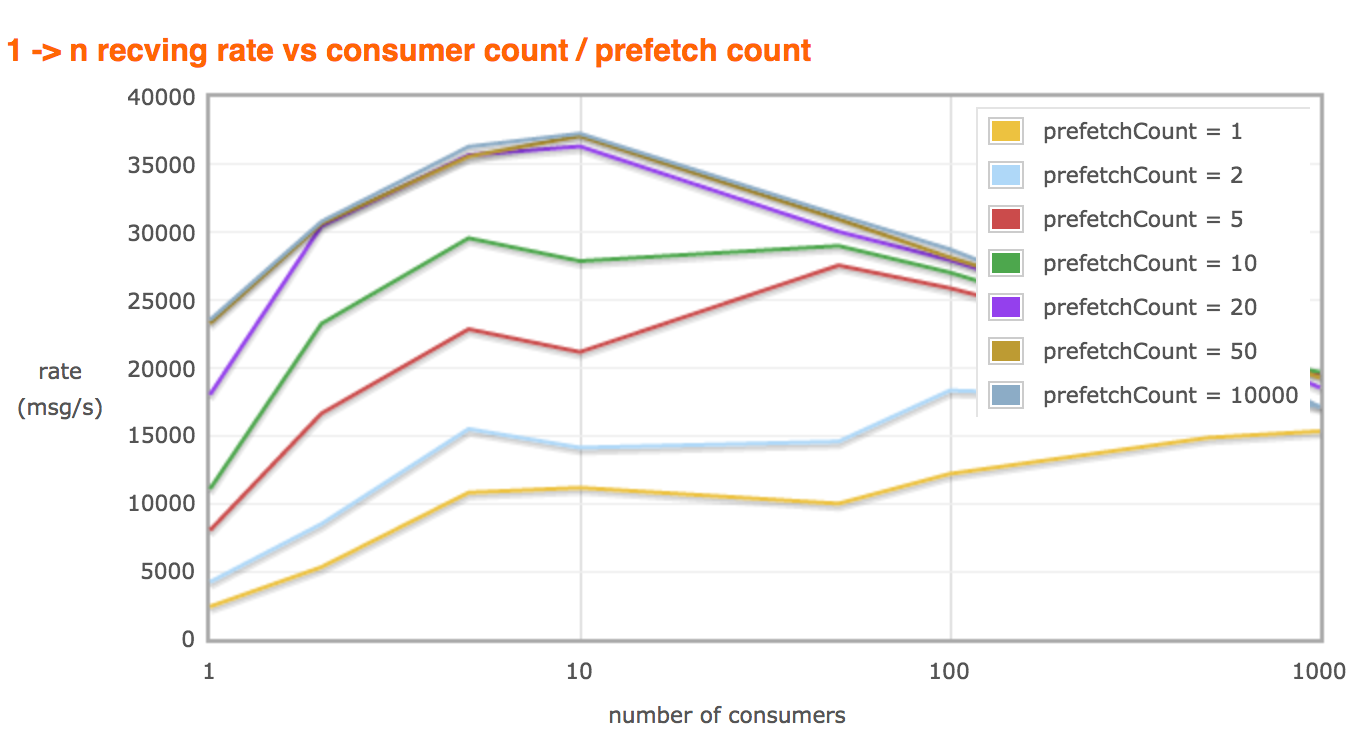
\includegraphics[width=1\textwidth]{figures/rabbitmqPrefetch}
  \caption[Chart showing performance variation when prefetch count is changed in the consumer]{Chart showing performance variation when prefetch count is changed in the consumer\footnotemark}
  \label{fig:rabbitmqBenchmark}
\end{figure}
\footnotetext{\fullcite{rabbitmqPerformance}}

\section{STOMP}
\label{sec:stomp}
  STOMP stands for Simple (or Streaming) Text Orientated Messaging Protocol. It is an alternative to other open messaging protocols such as AMQP. It provides an interoperable format for STOMP clients to communicate with a message broker system that supports STOMP. It provides interoperability among different languages, platforms and brokers.~\cite{stomp}
  STOMP is designed to be a lightweight protocol that is easy to implement in both client and server.
  \subsection{Protocol Overview}
  STOMP is a frame based protocol. A frame consists of a command, a set of optional headers and an optional body. STOMP is text based but it allows the transmission of binary messages~\cite{stomp}.
  A STOMP client can either be producer or consumer. As a producer  a message can be sent to a destination to server using SEND frame. Meanwhile, as a consumer, SUBSCRIBE frame should be sent for subscription of a message for a given destination. Then, the messages are received as MESSAGE frames.

  \subsection{STOMP Library for Dart}
  \label{subsec:stompForDart}
  Given that dart is a fairly new language, there is no AMQP client for RabbitMQ yet. As mentioned above in section~\ref{sec:rabbitmq} RabbitMQ also supports STOMP. An open source STOMP client\footnote{https://github.com/rikulo/stomp} in dart is available created by ‘Potix corporation’. It can perform most of the basic operations with message broker system like connecting, creating queue, subscribing, enqueuing and dequeuing. Although it has those basic functionalities, it still has some limitations and incompleteness like lack of support of ‘Heartbeat’ and it only supports STOMP version 1.2 or above.


\section{WebSocket}
  WebSocket protocol enables two-way communication between client and server over a single TCP connection. It uses origin-based security model, which is found in web browsers. It can be used for variety of web applications: games, stock tickers, multiuser applications, user interfaces exposing server-side services in real time, etc.~\cite{rfc6455}

  Since, HTTP was not initially designed for bidirectional communication, the WebSocket Protocol is designed to displace other existing bidirectional communication technologies that are based on HTTP~\cite{rfc6455}.

  WebSocket uses two URI schemes: “ws://” for normal WebSocket connection and “wss://” for secured WebSocket connection~\cite{rfc6455}.

\subsection{Security}
  The WebSocket Protocol uses the origin model used by web browsers to restrict which web pages can contact a WebSocket server when the WebSocket Protocol is used from a web page~\cite{rfc6455}.

   A WebSocket server reads the handshake sent by client to establish a connection. Thus, an attempt to connection to WebSocket from other protocols cannot succeed if it is not sent by a WebSocket client.~\cite{rfc6455}

\subsection{Establishing a Connection}
  When establishing a WebSocket connection, the HTTP server receives a regular GET request with an offer to upgrade to WebSocket. The server responds to the request to complete the handshake and establish the connection. Then the communication takes place in full-duplex mode~\cite{rfc6455}.
  
